\section{Diskretizacija problema}

Večina literature iz teorije \texttt{FEM} obravnava skalarne funkcije s stališča funkcionalne analize - kot vektorje. Enačbe iz prejšnjega poglavja bi v takšnem zapisu izgledale preprosteje. Omenjen pristop bi dodal novo plast konceptov, ki bi jih moral bralec predhodno razumeti, zato smo se ga za zaćetek izognili. Eden takšnih konceptov je koncept prostostnih stopenj funkcije. Razlaga diskretizacije problema je brez njega precej otežena, zato bomo tukaj na hitro opisali bistvo vektorske obravnave funkcij.

V znanem 3D vektorskem prostoru so osnovni gradniki trije bazni vektorji. S takšnim prostorom lahko opišemo vse možne diskretne skalarne funkcije, katerih domena sestoji le iz treh točk (slika \ref{fig:discreteExample}a). Vsaka konfiguracija treh skalarjev ustreza eni točki v našem 3D prostoru, ki ga posledično imenujemo funkcijski prostor. Dimenzija funkcijskega prostora je torej povezana z gostoto vzorčenja domene. Če na domeno postavimo trinajst točk (slika \ref{fig:discreteExample}b), bomo za opis vseh možnih konfiguracij potrebovali trinajst-dimenzionalni vektorski prostor. Če na domeno postavimo neskončno točk, kar storimo pri obravnavi zveznih funkcij (slika \ref{fig:discreteExample}c), bomo potrebovali neskončno dimenzionalni vektorski prostor. In kaj so potem bazni vektorji našega prostora? To so $\delta$ funkcije, postavljene v ustreznih točkah domene.

\begin{figure}[ht]
   \centering
   \begin{subfigure}[b]{0.32\textwidth}
      \centering
      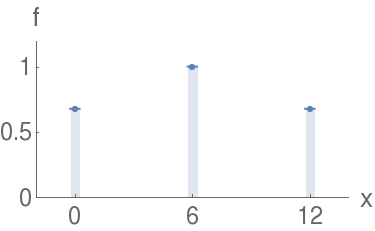
\includegraphics[width=0.94\textwidth]{Slike/discreteExample}
      \vspace{0mm}
      \caption{}
   \end{subfigure}
   \hspace{0mm}
   \begin{subfigure}[b]{0.32\textwidth}
      \centering
      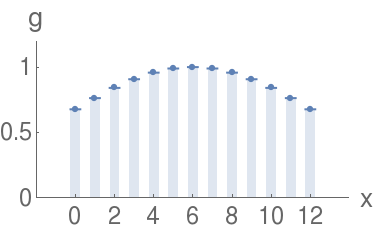
\includegraphics[width=0.94\textwidth]{Slike/discreteExample2}
      \caption{}
   \end{subfigure}
   \hspace{0mm}
   \begin{subfigure}[b]{0.32\textwidth}
      \centering
      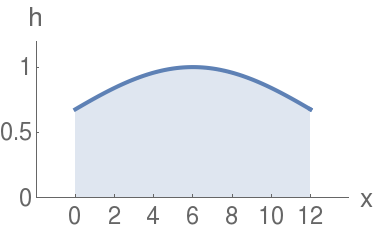
\includegraphics[width=0.94\textwidth]{Slike/discreteExample3}
      \caption{}
   \end{subfigure}
   \caption{Funkcije, ki živijo v (a) 3D, (b) 13D in (c) $\infty$-D funkcijskem (vektorskem) prostoru.}
   \label{fig:discreteExample}
\end{figure}

Na dimenzije vektorja gledamo kot na \textbf{prostostne stopnje}, katerih vrednosti lahko poljubno nastavljamo. Funkcijo $f$ (slika \ref{fig:discreteExample}a) zapišemo s komponentami in baznimi vektorji kot:
\begin{equation}
   \ket{f} =
   \begin{pmatrix}
      \mkern1mu 0,68 & 1,00, & 0,68 \mkern1mu
   \end{pmatrix}
   \begin{pmatrix}
      \mkern1mu \delta(x) \\
      \delta(x-6)         \\
      \delta(x-12) \mkern1mu
   \end{pmatrix}
   =
   \mkern2mu 0,68 \, \delta(x) + 1,00 \, \delta(x-6) + 0,68 \, \delta(x-12)
   \ ,
   \label{eq:discreteF}
\end{equation}
Funkcijo $g$ (slika \ref{fig:discreteExample}b) zapišemo s komponentami in baznimi vektorji kot:
\begin{equation}
   \ket{g} =
   \begin{pmatrix}
      \mkern1mu 0,68 & 0,76 & \cdots & 0,68 \mkern1mu
   \end{pmatrix}
   \begin{pmatrix}
      \delta(x)   \\
      \delta(x-1) \\
      \vdots      \\
      \delta(x-12)
   \end{pmatrix}
   =
   \mkern2mu 0,68 \, \delta(x) + 0,76 \, \delta(x-1) + ... + 0,68 \, \delta(x-12)
   \ .
   \label{eq:discreteG}
\end{equation}
Še vedno veljajo vsa pravila vektorskih prostorov. Tako je na primer skalarni produkt funkcije $\ket{f}$ same s seboj enak:
\begin{equation}
   \bra{f}\ket{f} =
   \begin{pmatrix}
      \mkern1mu 0,68 & 1,00, & 0,68 \mkern1mu
   \end{pmatrix}
   \begin{pmatrix}
      0,68 \\
      1,00 \\
      0,68
   \end{pmatrix}
   =
   1,92 \ .
\end{equation}
Skalarni produkt je definiran le za funkciji znotraj istega funkcijskega prostora. Pri zvezni funkciji $h$ (slika \ref{fig:discreteExample}c) komponent in baznih vektorjev ne moremo našteti, ker jih je neštevno neskončno. Kljub temu lahko funkcijski vektor izrazimo analogno, kot smo to storili v diskretnih primerih \eqref{eq:discreteF} in \eqref{eq:discreteG}. Diskretno vsoto členov pretvorimo v zvezno vsoto (integral):
\begin{equation}
   \ket{h} = \int_{0}^{12} h(x_0) \mkern3mu \delta(x-x_0) \mkern5mu \text{d}x_0 = h(x) \text{ na območju } x \in [0, 12] \ .
\end{equation}
Skalarni produkt dveh zveznih funkcij je po analogiji enak:
\begin{equation}
   \bra{h}\ket{h} =
   \int_0^{12} h(x) \mkern2mu h(x) \mkern5mu \text{d}x \ .
\end{equation}
Če skalarne funkcije predstavimo kot funkcijske vektorje, kako potem na isti način predstavimo vektorske funkcije (ki slikajo v več skalarnih spremenljivk)? Tako, da vsako komponento (skalarno funkcijo) posebej zapišemo kot funkcijski vektor. Tako dobimo vektor vektorjev, oz. matriko. Zdaj vidimo, zakaj smo temelje \texttt{FEM} opisali brez uporabe omenjenih konceptov. Zahtevnost zapisov enačb se zmanjša na račun povečane zahteve po predstavljivosti zapisov. Kot primer v novem jeziku zapišimo variacijsko izjavo \eqref{eq:LsfemVariationalStatement}:
\begin{equation}
   \bra{\mkern1mu \mathbsf{A} \! \cdot \! \mathbf{v} \mkern2mu}\ket{\mkern2mu \mathbsf{A} \! \cdot \! \mathbf{u} - \mathbf{f}\mkern1mu} \ = \,
   0 \ , \hspace{5mm} \forall \mathbf{v} \ .
   \label{eq:LsfemVariationalStatementNew}
\end{equation}
To izgleda veliko bolje, kajne?

Za numerično reševanje problema moramo abs\-trakt\-no zastavitev \eqref{eq:LsfemVariationalStatement} z neskončno prostostnimi stop\-nja\-mi diskretizirati. Iskanje želimo omejiti na $N$ čim enakomerneje razporejenih točk, ki jih imenujemo \textbf{vozlišča}. V vsako vozlišče postavimo \textbf{vozliščno bazno funkcijo}, ki pokrije le okolico vozlišča:
\begin{IEEEeqnarray*}{rc}
   \hspace{16mm} \ket{\Phi_i} \, , \hspace{5mm} i = 1, ..., N \hspace{16mm} & \texttt{vozliščne funkcije .}
\end{IEEEeqnarray*}
Neskončno število neskončno ozkih stolpičev smo zamenjali s končnim številom ($N$) končno ozkih grbin. Problemu omejimo število prostostnih stopenj tako, da dopustimo le obstoj tistih funkcij $v(\mathbf{x})$, ki so superpozicija vozliščnih funkcij. To so funkcije, ki jih lahko zapišemo kot vrsto vozliščnih funkcij $\Phi_i(\mathbf{x})$ s koeficienti $v_i$:
\vspace{-3mm}
\begin{equation}
   \ket{v} = \sum_{i = 1}^N v_i \ket{\Phi_i} \ .
   \label{eq:nodalSeries}
\end{equation}
S tem problem prevedemo na iskanje $N$ \textbf{vozliščnih vrednosti} $v_i$. Naslikajmo idejo na skrajno preprosti kvadratni domeni $[-3,\mkern2mu 3\mkern1mu] \mkern-1mu \times \mkern-1mu [-3,\mkern2mu 3\mkern1mu]$ s krajevnim vektorjem $\bm{\chi} = \{\xi,\eta\}$. Nanjo postavimo pravokotno mrežo s šestnajstimi vozlišči (slika \ref{fig:regionAndNodeFunctions}a) in nad njimi napnemo prav toliko vozliščnih funkcij z nastavljivimi višinami $v_i\mkern1mu$ (slika \ref{fig:regionAndNodeFunctions}b).

\begin{figure}[ht]
   \centering
   \begin{subfigure}[b]{0.42\textwidth}
      \centering
      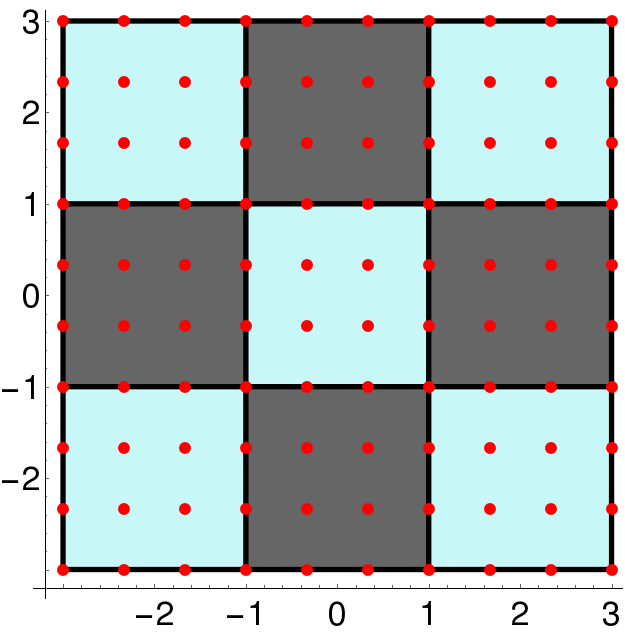
\includegraphics[width=0.94\textwidth]{Slike/layout2d}
      \vspace{0mm}
      \caption{}
   \end{subfigure}
   \hspace{5mm}
   \begin{subfigure}[b]{0.42\textwidth}
      \centering
      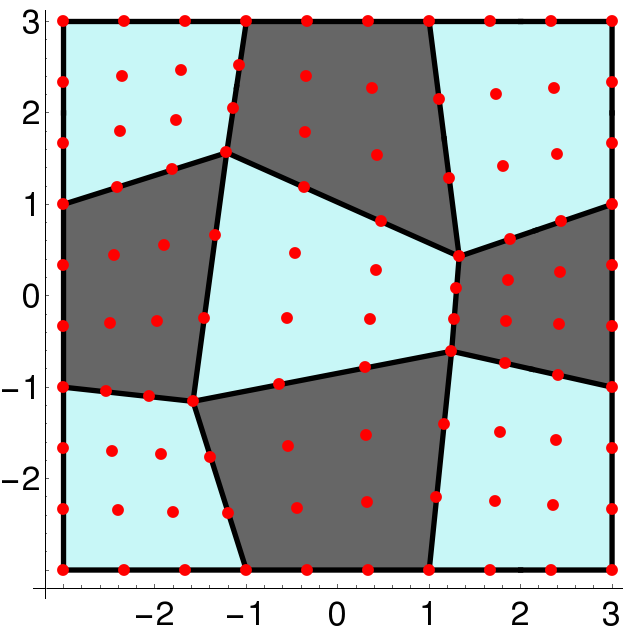
\includegraphics[width=0.94\textwidth]{Slike/layout2dTrans}
      \caption{}
   \end{subfigure}
   \caption{(a) Pravokotna domena z devetimi elementi (modre številke) in šestnajstimi vozlišči (rdeče številke) ter (b) nad vozlišči napete vozliščne funkcije. V prid nazornosti rišemo le štiri osrednje vozliščne funkcije.}
   \label{fig:regionAndNodeFunctions}
\end{figure}

\begin{figure}[ht]
   \centering
   \begin{subfigure}[b]{0.48\textwidth}
      \centering
      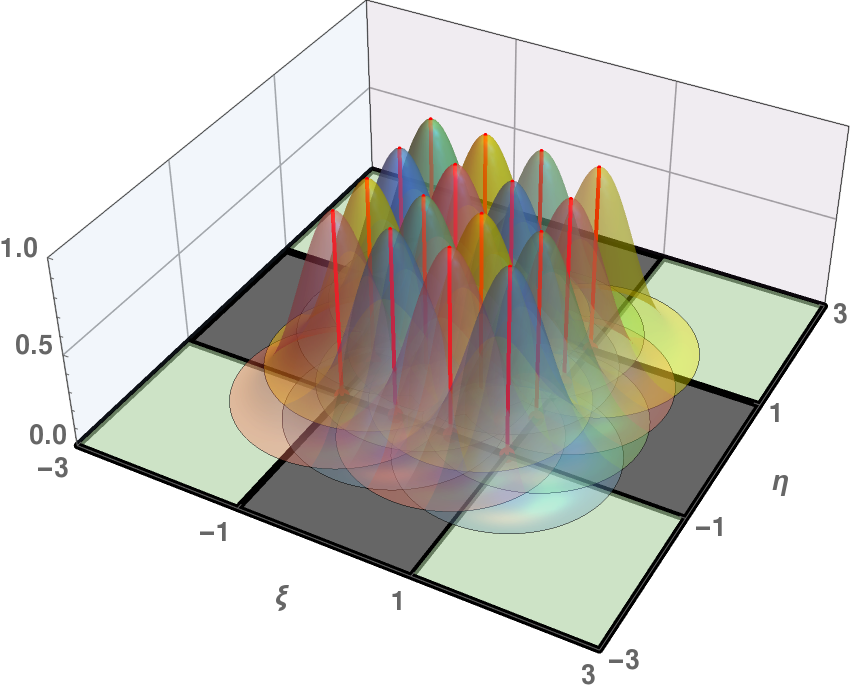
\includegraphics[width=0.94\textwidth]{Slike/nodalFuncs3d}
      \vspace{0mm}
      \caption{}
   \end{subfigure}
   \begin{subfigure}[b]{0.46\textwidth}
      \centering
      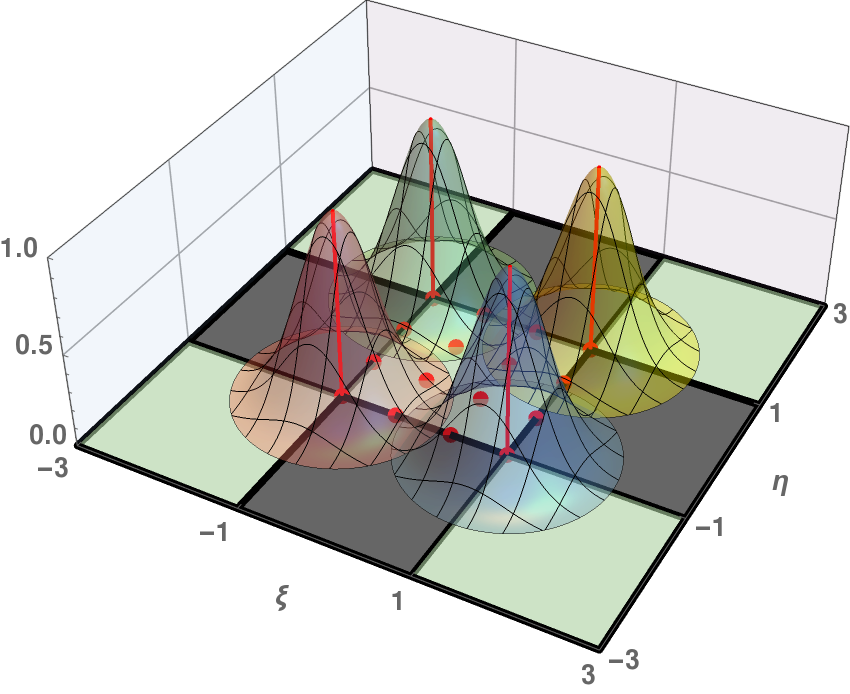
\includegraphics[width=0.94\textwidth]{Slike/nodalFuncs3dSparse}
      \caption{}
   \end{subfigure}
   \caption{}
   \label{fig:nodalFs}
\end{figure}

Štirikotne ploskvice, ki nastanejo s postavitvijo vozlišč, imenujemo \textbf{elementi}. Nobena vozliščna funkcija $\Phi_i$ ne sme pokrivati elementov, ki niso v stiku z njenim vozliščem. S tem dosežemo, da je $v(\bm\chi)$ nad nekim elementom sestavljena le iz funkcij v neposredni bližini tega elementa. Tako je $\mathbf{v}(\bm\chi)$ na sliki \ref{fig:sumAndShapeFunctions}a nad osrednjim elementom popolnoma določena z vrednostmi $v_6, v_7, v_{10}$ in $v_{11}$.

Ozrimo se na variacijsko izjavo \eqref{eq:LsfemVariationalStatement} ter si predstavljajmo funkcije $\mathbsf{A}(\mathbf{x}), \mathbf{u(x)}, \mathbf{v(x)}$ in $\mathbf{f(x)}$ zapisane v smislu razvoja po vozliščnih funkcijah \eqref{eq:nodalSeries}. Zaslutimo, da bomo računali prekrivne integrale vozliščnih funkcij:
\begin{equation}
   \bra{\Phi_i}\ket{\Phi_j} \ .
\end{equation}
To je enostavno dokler so vsi elementi iste oblike in velikosti, kot na sliki \ref{fig:regionAndNodeFunctions}. Takrat je dovolj, da izračunamo prekrivne integrale za vozlišča enega elementa. Kaj pa, če želimo uporabljati elemente poljubne oblike? Kako naj čim učinkoviteje, če so elementi poljubne oblike

Segmente vozliščnih funkcij $\Phi_6, \, \Phi_7, \, \Phi_{10}$ in $\Phi_{11}$, ki se nahajajo neposredno nad elementom 5, proglasimo za \textbf{elementarne funkcije} $\phi_{5 j}(\bm\chi)$ tega elementa (slika \ref{fig:sumAndShapeFunctions}b). Tako lahko funkcijo $\mathbf{v}$ na

\begin{figure}[ht]
   \centering
   \begin{subfigure}[b]{0.48\textwidth}
      \centering
      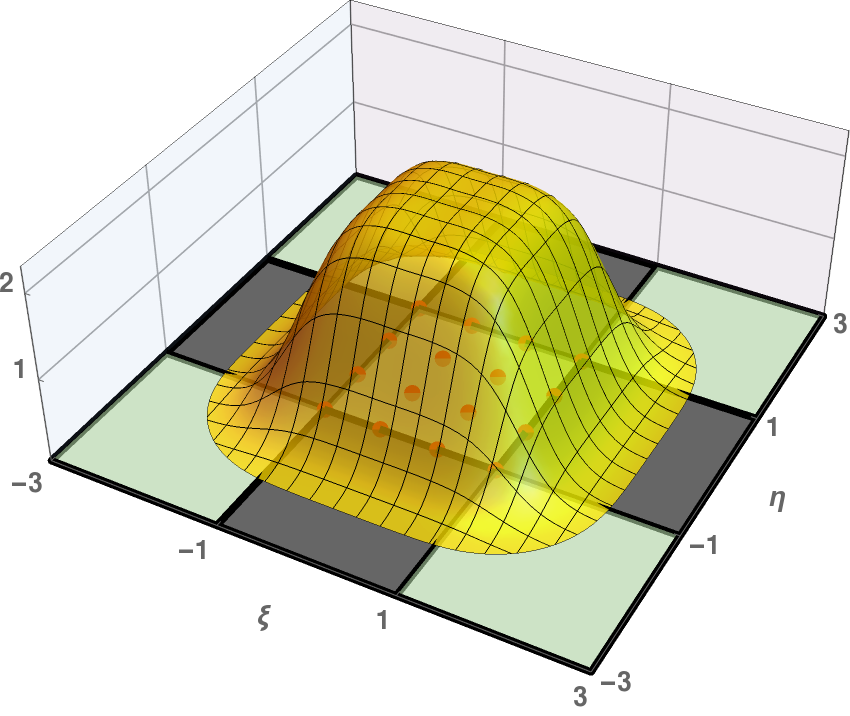
\includegraphics[width=0.94\textwidth]{Slike/nodalFuncsSumOverElm}
      \vspace{0mm}
      \caption{}
   \end{subfigure}
   \begin{subfigure}[b]{0.48\textwidth}
      \centering
      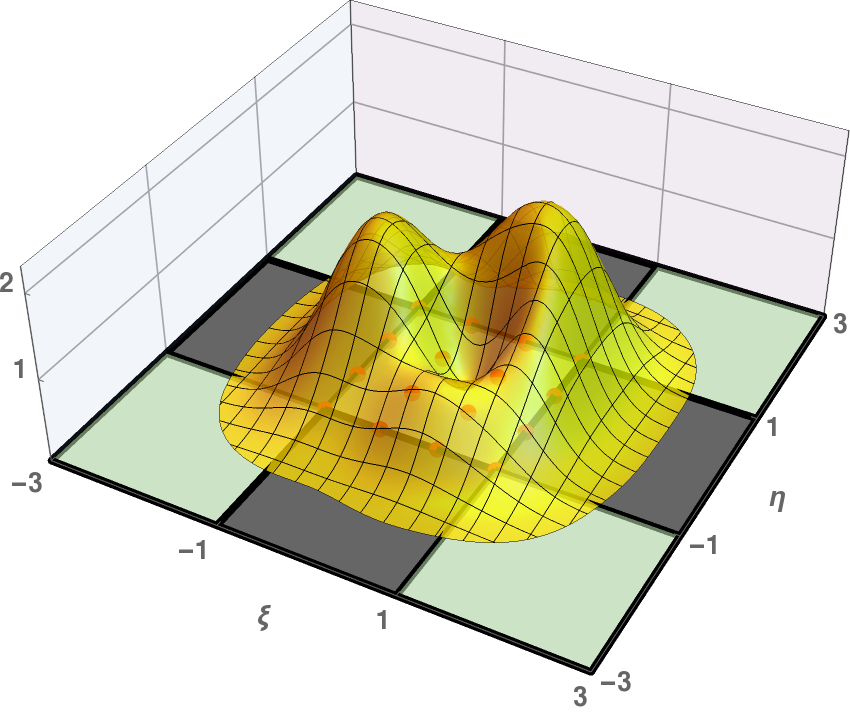
\includegraphics[width=0.94\textwidth]{Slike/nodalFuncsSumOverElmMod}
      \caption{}
   \end{subfigure}
   \caption{(a) vsota vozliščnih funkcij s slike \ref{fig:regionAndNodeFunctions}b in (b) elementarne funkcije, ki pripadajo elementu 5.}
   \label{fig:sumAndShapeFunctions}
\end{figure}

\begin{figure}[ht]
   \centering
   \begin{subfigure}[b]{0.44\textwidth}
      \centering
      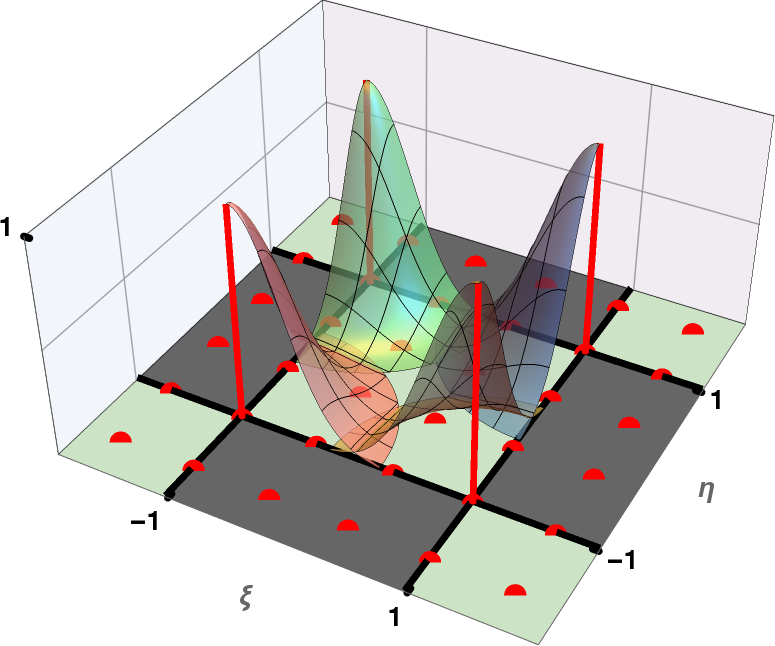
\includegraphics[width=0.94\textwidth]{Slike/elmFuncs3d}
      \vspace{0mm}
      \caption{}
   \end{subfigure}
   \hspace{3mm}
   \begin{subfigure}[b]{0.45\textwidth}
      \centering
      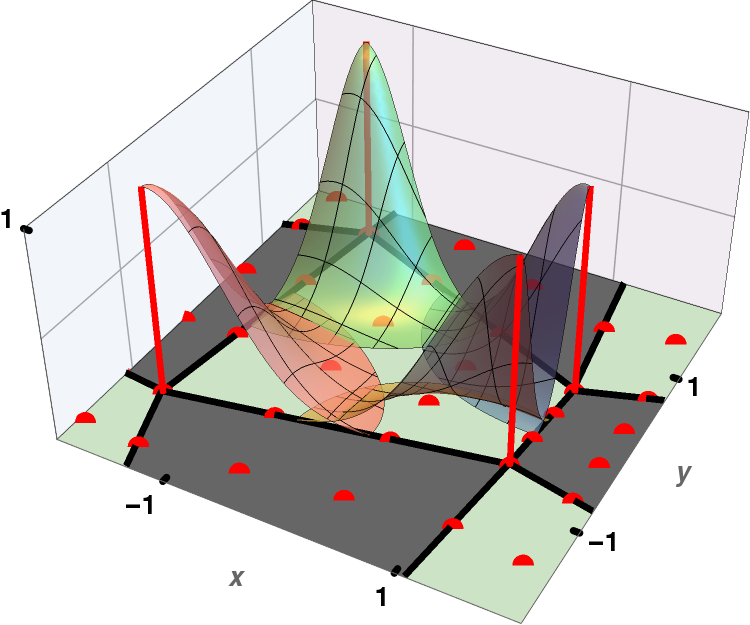
\includegraphics[width=0.94\textwidth]{Slike/elmFuncs3dTrans}
      \caption{}
   \end{subfigure}
   \caption{}
   \label{fig:shapeFs}
\end{figure}

še vedno  Z natančno analitično izpeljavo se prebijemo do izjave \eqref{eq:LsfemVariationalStatement}, od tod dalje pa moramo iskanje funkcije $\mathbf{u(x)}$ z neskončno prostostnimi stopnjami poenostaviti v iskanje funkcije s končnim številom prostostnih stopenj $N$.

Skozi oči \texttt{FI} je $\ket{\Phi_i}$ eden izmed baznih vektorjev v razvoju vektorja $\ket{v}$, $v_i$ pa pripadajoča komponenta.
V jeziku funkcionalne analize (\texttt{FI}) pravimo, da smo omejili funkcijski prostor.

nadaljujemo z diskretizacijo problema, to je, pretvorbo na sistem $N$ algebrajskih enačb. Ta korak je enak pri vseh različicah \texttt{FEM}. Funkcije na domeni $\Omega$ imajo neskončno štveilo prostostnih stopenj.
\begin{equation}
   u_i(\mathbf{x}) = \sum_{a = 1}^N \Phi^{a0} u^{a0}_i
\end{equation}

Mreža je v tem šolskem primeru strukturirana, kar pomeni, da je razporeditev elementov Kartezična. Mreža je lahko pri \texttt{FEM} tudi nestrukturirana, kar je ena izmed prednosti metode.

Naj bodo:
\begin{equation}
   \mathbf{T_1} = (x_1,y_1), \quad \mathbf{T_2} = (x_2,y_2), \quad \mathbf{T_3} = (x_3,y_3), \quad \mathbf{T_4} = (x_4,y_4)
\end{equation}
oglišča pravega elementa. Imejmo preslikavo $\mathbf{r}(\bm{\chi})$, ki slika iz referenčnega kvadrata $\bm{\chi}$ v realni prostor $\mathbf{x}$:
\begin{equation}
   \mathbf{r}(\bm{\chi})
   =
   \begin{pmatrix}
      x(\bm{\chi}) \\
      y(\bm{\chi})
   \end{pmatrix}
   =
   \begin{pmatrix}
      x_1 S_1(\bm{\chi}) + x_2 S_2(\bm{\chi}) + x_3 S_3(\bm{\chi}) + x_4 S_4(\bm{\chi}) \\
      y_1 S_1(\bm{\chi}) + y_2 S_2(\bm{\chi}) + y_3 S_3(\bm{\chi}) + y_4 S_4(\bm{\chi})
   \end{pmatrix} \ ,
\end{equation}
kjer so $S_i$ ogliščne funkcije:
\begin{equation}
   \mathbf{S}
   =
   \begin{pmatrix}
      (1+\xi)(1+\eta) \\
      (1+\xi)(1-\eta) \\
      (1-\xi)(1+\eta) \\
      (1-\xi)(1-\eta)
   \end{pmatrix}
\end{equation}
ali kompaktneje:
\begin{equation}
   \begin{pmatrix}
      x(\bm{\chi}) \\
      y(\bm{\chi})
   \end{pmatrix}
   =
   \begin{pmatrix}
      x_1 & x_2 & x_3 & x_4 \\
      y_1 & y_2 & y_3 & y_4
   \end{pmatrix}
   \begin{pmatrix}
      S_1(\bm{\chi}) \\
      S_2(\bm{\chi}) \\
      S_3(\bm{\chi}) \\
      S_4(\bm{\chi})
   \end{pmatrix} \ .
\end{equation}
Jakobijevka preslikave $\mathbf{r}(\bm{\chi})$ je enaka:
\begin{equation}
   \mathbsf{J}
   =
   \begin{pmatrix}
      \frac{\pd x}{\pd \xi} & \frac{\pd x}{\pd \eta} \\
      \frac{\pd y}{\pd \xi} & \frac{\pd y}{\pd \eta}
   \end{pmatrix} \ .
\end{equation}
$\psi$ in $\phi$ sta skalarni funkciji. $\bar{\texttt{J}}$ je inverz Jakobijevke:
\begin{equation}
   \mathbf{\nabla_{\mkern-3mu x}} \psi(\mathbf{x}) = \bar{\mathbsf{J}} \mkern3mu \mathbf{\nabla_{\mkern-4mu \chi}} \phi(\bm{\chi}) \ .
\end{equation}
$\bar{\texttt{J}}$ je enak:
\begin{equation}
   \bar{\mathbsf{J}}
   =
   \frac{1}{\det \mathbsf{J}}
   \begin{pmatrix}
      +J_{22} & -J_{12} \\
      -J_{21} & +J_{11}
   \end{pmatrix}
   \ .
\end{equation}
Odvod $\psi$ po $x_1$ označimo kot $\psi^1$:
\begin{equation}
   \psi^1 = \left(\bar{J}_{11} \phi^1 + \bar{J}_{12} \phi^2 \right) \ .
\end{equation}
Zapisano na konvencionalen način:
\begin{equation}
   \left(\frac{\pd \psi}{\pd x}\right)_{\mkern-4mu y}
   =
   \bar{J}_{11} \mkern-2mu \left(\frac{\pd \phi}{\pd \xi}\right)_{\mkern-3mu \eta}
   +
   \bar{J}_{12} \mkern-2mu \left(\frac{\pd \phi}{\pd \eta}\right)_{\mkern-3mu \xi} \ ,
\end{equation}
oziroma:
\begin{equation}
   \left(\frac{\pd \psi}{\pd x} \right)_{\mkern-3mu y}
   =
   \left(\frac{\pd \xi}{\pd x} \right)_{\mkern-4mu y}
   \mkern-4mu \left(\frac{\pd \phi}{\pd \xi}\right)_{\mkern-3mu \eta}
   +
   \left(\frac{\pd \eta}{\pd x}\right)_{\mkern-4mu y}
   \mkern-4mu \left(\frac{\pd \phi}{\pd \eta}\right)_{\mkern-3mu \xi}
\end{equation}
Če definiramo:
\begin{equation}
   \mathbsf{\mathfrak{J}}
   =
   \frac{1}{\det \mathbsf{J}}
   \begin{pmatrix}
      \det \mathbsf{J} & 0       & 0       \\
      0                & +J_{22} & -J_{12} \\
      0                & -J_{21} & +J_{11}
   \end{pmatrix} \ ,
\end{equation}
lahko zapišemo:
\begin{equation}
   \psi^p = \mathfrak{J}_{pq} \phi^{q} \ .
   \label{eq:refToEmt}
\end{equation}
Po vozliščih $(a, b, c, d \in [1,N])$:
\begin{equation}
   \braket{
      \left(A^{b p}_{\mkern14mu hk} \mkern1mu \Psi_b \frac{\pd}{\pd x_p}\right)
      \left(v^{\mkern1mu i}_{\triangleright \mkern1mu k} \mkern1mu \Psi_i \right)}
   {
      \left(A^{c q h l} \mkern1mu \Psi_c \frac{\pd}{\pd x_q}\right)
      \left(u^{j l}_\triangleright \mkern1mu \Psi_j + u^{j l}_\triangleleft \mkern1mu \Psi_j \right)
      -
      f^{c h}_{\bowtie} \mkern1mu \Psi_c }
\end{equation}
Po elementih $(\alpha, \beta, \gamma, \delta) \in [1,12]$, kjer je $n$ število elementov.
\begin{equation}
   \sum^n_{\varepsilon}
   \braket{
      \left(A^{\substack{\mkern2mu \varepsilon \\[0.15mm] \beta} \mkern2mu p}_{\mkern19mu hk} \mkern2mu \psi_{ \varepsilon \beta} \frac{\pd}{\pd x_p}\right) \mkern-5mu
      \left(v^{\mkern 2mu \substack{\varepsilon \\[-0.5mm] \alpha \\[-0.2mm]}}_{\triangleright \mkern5mu k} \mkern2mu \psi_{\varepsilon \alpha}\right)}
   {
      \left(A^{\substack{\mkern2mu \varepsilon \\[-0.4mm] \gamma} \mkern2mu qhl} \mkern2mu \psi_{\varepsilon \gamma} \frac{\pd}{\pd x_q}\right) \mkern-5mu
      \left(u^{\substack{\mkern2mu \varepsilon \\[0.2mm] \delta} \mkern2mu l}_\triangleright \psi_{\varepsilon \delta} + u^{\substack{\mkern2mu \varepsilon \\[0.2mm] \delta} \mkern2mu l}_\triangleleft \psi_{\varepsilon \delta} \right)
      -
      f^{\substack{\mkern2mu \varepsilon \\[-0.4mm] \gamma} \mkern2mu h}_{\bowtie} \mkern1mu \psi_{\varepsilon \gamma}}
\end{equation}
Uporabimo parcialni diferencialni operator (absorbiramo indeks v naslednji oklepaj):
\begin{equation*}
   \sum^n_\varepsilon
   \braket{
      \left( A^{\substack{\mkern2mu \varepsilon \\[0.15mm] \beta} \mkern2mu p}_{\mkern19mu hk} \mkern2mu \psi_{ \varepsilon \beta 0} \right) \mkern-2mu
      v^{\mkern 2mu \substack{\varepsilon \\[-0.5mm] \alpha \\[-0.2mm]}}_{\triangleright \mkern5mu k} \mkern2mu \psi_{\varepsilon \alpha p} \mkern4mu}
   {
      \mkern2mu \left( A^{\substack{\mkern2mu \varepsilon \\[-0.4mm] \gamma} \mkern2mu qhl} \mkern2mu \psi_{\varepsilon \gamma 0} \right) \mkern-5mu 
      \left( u^{\substack{\mkern2mu \varepsilon \\[0.2mm] \delta} \mkern2mu l}_\triangleright \psi_{\varepsilon \delta q} + u^{\substack{\mkern2mu \varepsilon \\[0.2mm] \delta} \mkern2mu l}_\triangleleft \psi_{\varepsilon \delta q} \right)
      -
      f^{\substack{\mkern2mu \varepsilon \\[-0.4mm] \gamma} \mkern2mu h}_{\bowtie} \mkern1mu \psi_\gamma }
\end{equation*}
Preuredimo:
\begin{equation*}
   \sum^n_\varepsilon
   v^{\mkern 2mu \substack{\varepsilon \\[-0.5mm] \alpha \\[-0.2mm]}}_{\triangleright \mkern5mu k} \mkern2mu A^{\substack{\mkern2mu \varepsilon \\[0.15mm] \beta} \mkern2mu p}_{\mkern19mu hk}
   \braket{
      \psi_{ \varepsilon \beta 0} \psi_{\varepsilon \alpha p} }
   {
      \mkern2mu A^{\substack{\mkern2mu \varepsilon \\[-0.4mm] \gamma} \mkern2mu qhl}     \psi_{\varepsilon \gamma 0} \mkern2mu     u^{\substack{\mkern2mu \varepsilon \\[0.2mm] \delta} \mkern2mu l}_\triangleright     \psi_{\varepsilon \delta q}
      +
      A^{\substack{\mkern2mu \varepsilon \\[-0.4mm] \gamma} \mkern2mu qhl}    \psi_{\varepsilon \gamma 0} \mkern2mu     u^{\substack{\mkern2mu \varepsilon \\[0.2mm] \delta} \mkern2mu l}_\triangleleft \psi_{\varepsilon \delta q}
      -
      f^{\substack{\mkern2mu \varepsilon \\[-0.4mm] \gamma} \mkern2mu h}_{\bowtie} \mkern1mu    \psi_{\varepsilon \gamma 0} }
\end{equation*}
Kar lahko, postavimo izven integrala:
\begin{equation*}
   \sum^n_\varepsilon   v^{\mkern 2mu \substack{\varepsilon \\[-0.5mm] \alpha \\[-0.2mm]}}_{\triangleright \mkern5mu k} \left(
   \left\langle   \psi_{ \varepsilon \beta 0} \mkern1mu    \psi_{\varepsilon \alpha p} \mkern1mu    \psi_{\varepsilon \gamma 0} \mkern1mu    \psi_{\varepsilon \delta q}   \right\rangle
   A^{\substack{\mkern2mu \varepsilon \\[0.15mm] \beta} \mkern2mu p}_{\mkern19mu hk}    A^{\substack{\mkern2mu \varepsilon \\[-0.4mm] \gamma} \mkern2mu qhl} \mkern1mu     u^{\substack{\mkern2mu \varepsilon \\[0.2mm] \delta} \mkern2mu l}_\triangleright
   +
   \left\langle    \psi_{ \varepsilon \beta 0} \mkern1mu    \psi_{\varepsilon \alpha p} \mkern1mu    \psi_{\varepsilon \gamma 0} \mkern1mu    \psi_{\varepsilon \delta q}    \right\rangle
   A^{\substack{\mkern2mu \varepsilon \\[0.15mm] \beta} \mkern2mu p}_{\mkern19mu hk}    A^{\substack{\mkern2mu \varepsilon \\[-0.4mm] \gamma} \mkern2mu qhl}    u^{\substack{\mkern2mu \varepsilon \\[0.2mm] \delta} \mkern2mu l}_\triangleleft
   -
   \left\langle \psi_{ \varepsilon \beta 0} \mkern1mu    \psi_{\varepsilon \alpha p} \mkern1mu    \psi_{\varepsilon \gamma 0}    \right\rangle    A^{\substack{\mkern2mu \varepsilon \\[0.15mm] \beta} \mkern2mu p}_{\mkern19mu hk}    f^{\substack{\mkern2mu \varepsilon \\[-0.4mm] \gamma} \mkern2mu h}_{\bowtie}
   \right)
\end{equation*}
Definiramo tenzorja $\mathbsf{S}$ in $\mathbsf{T}$:
\begin{equation}
   S_{\varepsilon \beta \alpha p \gamma \delta q} = \left\langle   \psi_{ \varepsilon \beta 0} \mkern1mu    \psi_{\varepsilon \alpha p} \mkern1mu    \psi_{\varepsilon \gamma 0} \mkern1mu    \psi_{\varepsilon \delta q}   \right\rangle
\end{equation}
\begin{equation}
   T_{\varepsilon \beta \alpha p \gamma} = \left\langle \psi_{ \varepsilon \beta 0} \mkern1mu    \psi_{\varepsilon \alpha p} \mkern1mu    \psi_{\varepsilon \gamma 0}    \right\rangle \ .
\end{equation}
Tako imamo:
\begin{equation}
   \sum^n_\varepsilon v^{\mkern 2mu \substack{\varepsilon \\[-0.5mm] \alpha \\[-0.2mm]}}_{\triangleright \mkern5mu k} \left(
   S_{\varepsilon \beta \alpha p \gamma \delta q}    A^{\substack{\mkern2mu \varepsilon \\[0.15mm] \beta} \mkern2mu p}_{\mkern19mu hk}    A^{\substack{\mkern2mu \varepsilon \\[-0.4mm] \gamma} \mkern2mu qhl} \mkern1mu     u^{\substack{\mkern2mu \varepsilon \\[0.2mm] \delta} \mkern2mu l}_\triangleright
   +
   S_{\varepsilon \beta \alpha p \gamma \delta q}    A^{\substack{\mkern2mu \varepsilon \\[0.15mm] \beta} \mkern2mu p}_{\mkern19mu hk}    A^{\substack{\mkern2mu \varepsilon \\[-0.4mm] \gamma} \mkern2mu qhl}    u^{\substack{\mkern2mu \varepsilon \\[0.2mm] \delta} \mkern2mu l}_\triangleleft
   -
   T_{\varepsilon \beta \alpha p \gamma}    A^{\substack{\mkern2mu \varepsilon \\[0.15mm] \beta} \mkern2mu p}_{\mkern19mu hk}    f^{\substack{\mkern2mu \varepsilon \\[-0.4mm] \gamma} \mkern2mu h}_{\bowtie}
   \right) = 0 \ .
\end{equation}
Sestavitev globalnega tenzorja:
\begin{equation}
   \hspace{-10mm}
   \forall \, v^{ik}_{\triangleright}: \quad
   \sum^N_{i,j} \mkern-2mu v^{i k}_{\triangleright}
   \sum^n_\varepsilon
   \mkern-7mu
   \sum_{\substack{\alpha, \delta \, \ni: \\ (\varepsilon,\alpha) = i \\ (\varepsilon,\delta) = j}}^{12}
   \mkern-10mu
   \left(
   S_{\varepsilon \beta \alpha p \gamma \delta q} \mkern2mu
   A^{\substack{\mkern2mu \varepsilon \\[0.15mm] \beta} \mkern2mu p}_{\mkern19mu hk}    A^{\substack{\mkern2mu \varepsilon \\[-0.4mm] \gamma} \mkern2mu qhl} \mkern1mu     u^{\substack{\mkern2mu \varepsilon \\[0.2mm] \delta} \mkern2mu l}_\triangleright \right)
   =
   \sum^N_i v^{i k}_{\triangleright}
   \sum^n_\varepsilon
   \mkern-7mu
   \sum_{\substack{\alpha \, \ni: \\ (\varepsilon,\alpha) = i}}^{12}
   \mkern-10mu
   \left(
   T_{\varepsilon \beta \alpha p \gamma}
   A^{\substack{\mkern2mu \varepsilon \\[0.15mm] \beta} \mkern2mu p}_{\mkern19mu hk}    f^{\substack{\mkern2mu \varepsilon \\[-0.4mm] \gamma} \mkern2mu h}_{\bowtie}
   -
   S_{\varepsilon \beta \alpha p \gamma \delta q}    A^{\substack{\mkern2mu \varepsilon \\[0.15mm] \beta} \mkern2mu p}_{\mkern19mu hk}    A^{\substack{\mkern2mu \varepsilon \\[-0.4mm] \gamma} \mkern2mu qhl}    u^{\substack{\mkern2mu \varepsilon \\[0.2mm] \delta} \mkern2mu l}_\triangleleft
   \right)
\end{equation}
\begin{equation*}
   v^{i k}_{\triangleright} \left(
   K_{i k j l} \mkern1mu u^{j l}_\triangleright
   +
   G_{i k}
   -
   H_{i k}
   \right) = 0 \ .
\end{equation*}
\begin{equation*}
   F_{i k} = H_{i k} - G_{i k} \ .
\end{equation*}
\begin{equation*}
   v^{i k}_{\triangleright} \left(
   K_{i k j l} \mkern1mu u^{j l}_\triangleright
   -
   F_{i k}
   \right) = 0 \quad \forall v \ .
\end{equation*}
Končno:
\begin{equation}
   K_{i k j l} \mkern1mu u^{j l}_\triangleright
   =
   F_{i k} \ .
\end{equation}
Prekrivne integrale integriramo na referenčnem kvadratu:
\begin{equation}
   S_{\beta \alpha p \gamma \delta q} = \left\langle \phi^{\phantom{\beta}0}_\beta \mkern1mu ( \mathfrak{J}_{pr} \phi^{\phantom{\alpha}r}_\alpha ) \mkern1mu \phi^{\phantom{\gamma}0}_\gamma ( \mathfrak{J}_{qs}  \phi^{\phantom{\delta}s}_\delta ) \mkern2mu |\mkern-2mu \det \mathbsf{J}| \right\rangle_{\bm{\chi}}
\end{equation}
\begin{equation}
   T_{\beta \alpha p \delta} = \left\langle \phi^{\phantom{\beta}0}_\beta\mkern1mu ( \mathfrak{J}_{pr} \phi^{\phantom{\alpha}r}_\alpha ) \phi^{\phantom{\delta}0}_\delta \mkern2mu |\mkern-2mu \det \mathbsf{J}| \right\rangle_{\bm{\chi}} \ .
\end{equation}
Zapis, primeren za implementacijo:
\begin{equation}
   S_{\varepsilon \beta \alpha p \gamma \delta q}
   =
   \left\langle \phi^{\phantom{\beta}0}_\beta
   \mkern1mu
   ( \mathfrak{J}_{\varepsilon  pr}
   \phi^{\phantom{\alpha}r}_\alpha )
   \mkern1mu
   \phi^{\phantom{\gamma}0}_\gamma
   ( \mathfrak{J}_{\varepsilon qs}
   \phi^{\phantom{\delta}s}_\delta )
   \mkern2mu
   |\mathfrak{J}_{\varepsilon 00}| \right\rangle_{\bm{\chi}}
\end{equation}
\begin{equation}
   T_{\varepsilon \beta \alpha p \delta}
   =
   \left\langle \phi^{\phantom{\beta}0}_\beta
   \mkern1mu
   ( \mathfrak{J}_{\varepsilon pr}
   \phi^{\phantom{\alpha}r}_\alpha )
   \phi^{\phantom{\delta}0}_\delta
   \mkern2mu
   | \mathfrak{J}_{\varepsilon 00}| \right\rangle_{\bm{\chi}} \ .
\end{equation}
\begin{IEEEeqnarray*}{ccc}
   i, j & \ \rightarrow \ & \text{vozlišča od 1 do } N \\
   \varepsilon & \ \rightarrow \ & \text{elementi od 1 do } n, \\
   \alpha, \beta, \gamma, \delta & \ \rightarrow \ & \text{vozlišča v elementu od 1 do 12}, \\
   p, q, r, s & \ \rightarrow \ & \text{odvodi: 0 (id)}, 1 \ (\pd_x), \ 2 \ (\pd_y)
\end{IEEEeqnarray*}

Sprehodi se preko vseh točk in za vsako poišči vse asociirane pare $(i, a)$. Dva para za točke na stranici elementa, štirje pari za točke na ogliščih elementa. Vsota po $k$ v faktorju $v^a_k$ ima $m$ (število spremenljivk) seštevancev. Vsak seštevanec prispeva k vrstici globalne matrike. Seštevanci iz različnih asociiranih parov $(i, a)$ z istimi $k$ prispevajo k isti vrstici globalne matrike.

Podobno stori za asociirane pare $(i, d)$. Vsota po $l$ bo ponovno imela $m$ seštevancev. Seštevanci iz različnih asociiranih parov z istimi $l$ prispevajo k istemu stolpcu globalne matrike.

To pomeni \(2 \times 2 = 4\) prispevki za vsak element globalne matrike za točke na stranicah ali $4 \times 4 = 16$ za točke na ogliščih.

Lahko pa sestavljaš po elementih. $(i, a)$ določi pas vrstic, $k$ določi mesto znotraj pasu. $(i, d)$ določi pas stolpcev, $l$ pa mesto znotraj pasu.